% Options for packages loaded elsewhere
% Options for packages loaded elsewhere
\PassOptionsToPackage{unicode}{hyperref}
\PassOptionsToPackage{hyphens}{url}
%
\documentclass[
  10pt,
  ignorenonframetext,
  aspectratio=169,
  russian,
]{beamer}
\newif\ifbibliography
\usepackage{pgfpages}
\setbeamertemplate{caption}[numbered]
\setbeamertemplate{caption label separator}{: }
\setbeamercolor{caption name}{fg=normal text.fg}
\beamertemplatenavigationsymbolshorizontal
% remove section numbering
\setbeamertemplate{part page}{
  \centering
  \begin{beamercolorbox}[sep=16pt,center]{part title}
    \usebeamerfont{part title}\insertpart\par
  \end{beamercolorbox}
}
\setbeamertemplate{section page}{
  \centering
  \begin{beamercolorbox}[sep=12pt,center]{section title}
    \usebeamerfont{section title}\insertsection\par
  \end{beamercolorbox}
}
\setbeamertemplate{subsection page}{
  \centering
  \begin{beamercolorbox}[sep=8pt,center]{subsection title}
    \usebeamerfont{subsection title}\insertsubsection\par
  \end{beamercolorbox}
}
% Prevent slide breaks in the middle of a paragraph
\widowpenalties 1 10000
\raggedbottom
\AtBeginPart{
  \frame{\partpage}
}
\AtBeginSection{
  \ifbibliography
  \else
    \frame{\sectionpage}
  \fi
}
\AtBeginSubsection{
  \frame{\subsectionpage}
}
\usepackage{iftex}
\ifPDFTeX
  \usepackage[T1]{fontenc}
  \usepackage[utf8]{inputenc}
  \usepackage{textcomp} % provide euro and other symbols
\else % if luatex or xetex
  \usepackage{unicode-math} % this also loads fontspec
  \defaultfontfeatures{Scale=MatchLowercase}
  \defaultfontfeatures[\rmfamily]{Ligatures=TeX,Scale=1}
\fi
\usepackage{lmodern}

\usetheme[]{metropolis}
\usefonttheme{serif} % use mainfont rather than sansfont for slide text
\ifPDFTeX\else
  % xetex/luatex font selection
  \setmainfont[]{DejaVu Sans}
  \setsansfont[]{DejaVu Sans}
  \setmonofont[]{DejaVu Sans Mono}
\fi
% Use upquote if available, for straight quotes in verbatim environments
\IfFileExists{upquote.sty}{\usepackage{upquote}}{}
\IfFileExists{microtype.sty}{% use microtype if available
  \usepackage[]{microtype}
  \UseMicrotypeSet[protrusion]{basicmath} % disable protrusion for tt fonts
}{}


\usepackage{longtable,booktabs,array}
\newcounter{none} % for unnumbered tables
\usepackage{calc} % for calculating minipage widths
\usepackage{caption}
% Make caption package work with longtable
\makeatletter
\def\fnum@table{\tablename~\thetable}
\makeatother
\usepackage{graphicx}
\makeatletter
\newsavebox\pandoc@box
\newcommand*\pandocbounded[1]{% scales image to fit in text height/width
  \sbox\pandoc@box{#1}%
  \Gscale@div\@tempa{\textheight}{\dimexpr\ht\pandoc@box+\dp\pandoc@box\relax}%
  \Gscale@div\@tempb{\linewidth}{\wd\pandoc@box}%
  \ifdim\@tempb\p@<\@tempa\p@\let\@tempa\@tempb\fi% select the smaller of both
  \ifdim\@tempa\p@<\p@\scalebox{\@tempa}{\usebox\pandoc@box}%
  \else\usebox{\pandoc@box}%
  \fi%
}
% Set default figure placement to htbp
\def\fps@figure{htbp}
\makeatother



\ifLuaTeX
\usepackage[bidi=basic,shorthands=off,provide=*]{babel}
\else
\usepackage[bidi=default,shorthands=off,provide=*]{babel}
\fi
\ifPDFTeX
\else
\babelfont{rm}[]{DejaVu Sans}
\fi
\ifLuaTeX
  \usepackage{selnolig} % disable illegal ligatures
\fi


\setlength{\emergencystretch}{3em} % prevent overfull lines

\providecommand{\tightlist}{%
  \setlength{\itemsep}{0pt}\setlength{\parskip}{0pt}}



 

\usepackage[]{csquotes}

%%% Load theme
\IfFileExists{beamerthemegotham.sty}{
  %%%% Full TeXlive
  \usetheme{gotham}
  \gothamset{
    numbering=totalframenumber,
    parttocframe default=off,
    sectiontocframe default=off,
    subsectiontocframe default=off,
    tocframe template=gotham bullet,
    % progressbar position=frametitle,
    progressbar position=foot,
  }
  \renewcommand{\gothamInstituteLogoSquare}[1][4ex]{%
    
\includegraphics[height=##1]{_resources/image/logo_rudn-inverted.png}
  }
  % \renewcommand{\gothamtitlepagelogo}[1][4ex]{%
  %   
\includegraphics[height=##1]{_resources/image/logo_rudn.png}
  % }
}{%
  %%%% TinyTeX
  \usepackage{libertine}
  %%%% https://deic.uab.cat/~iblanes/beamer_gallery/
  \usetheme{Madrid}
}
\metroset{progressbar=frametitle,numbering=fraction}
\setbeamersize{text margin left=8mm,text margin right=8mm}
\makeatletter
\@ifpackageloaded{caption}{}{\usepackage{caption}}
\AtBeginDocument{%
\ifdefined\contentsname
  \renewcommand*\contentsname{Содержание}
\else
  \newcommand\contentsname{Содержание}
\fi
\ifdefined\listfigurename
  \renewcommand*\listfigurename{Список иллюстраций}
\else
  \newcommand\listfigurename{Список иллюстраций}
\fi
\ifdefined\listtablename
  \renewcommand*\listtablename{Список таблиц}
\else
  \newcommand\listtablename{Список таблиц}
\fi
\ifdefined\figurename
  \renewcommand*\figurename{Рисунок}
\else
  \newcommand\figurename{Рисунок}
\fi
\ifdefined\tablename
  \renewcommand*\tablename{Таблица}
\else
  \newcommand\tablename{Таблица}
\fi
}
\@ifpackageloaded{float}{}{\usepackage{float}}
\floatstyle{ruled}
\@ifundefined{c@chapter}{\newfloat{codelisting}{h}{lop}}{\newfloat{codelisting}{h}{lop}[chapter]}
\floatname{codelisting}{Список}
\newcommand*\listoflistings{\listof{codelisting}{Листинги}}
\makeatother
\makeatletter
\makeatother
\makeatletter
\@ifpackageloaded{caption}{}{\usepackage{caption}}
\@ifpackageloaded{subcaption}{}{\usepackage{subcaption}}
\makeatother

\usepackage{bookmark}
\IfFileExists{xurl.sty}{\usepackage{xurl}}{} % add URL line breaks if available
\urlstyle{same}
% fallback for those not using the hyperref driver hyperxmp:
\makeatletter
\@ifundefined{xmpquote}{\newcommand{\xmpquote}[1]{#1}}{}
\makeatother
\hypersetup{
  pdftitle={Лабораторная работа №6},
  pdfauthor={Нечаева Кира Андреевна},
  pdflang={ru-RU},
  hidelinks,
  pdfcreator={LaTeX via pandoc}}


\title{\texorpdfstring{Лабораторная работа №6}{Лабораторная работа №6}}
\subtitle{\texorpdfstring{Задача об эпидемии}{Задача об эпидемии}}
\author{Нечаева Кира Андреевна}
\date{}
\institute{НКНбд-01-23}

\begin{document}
\frame{\titlepage}


\begin{frame}{Постановка задачи}
\protect\phantomsection\label{ux43fux43eux441ux442ux430ux43dux43eux432ux43aux430-ux437ux430ux434ux430ux447ux438}
\textbf{Вариант 2}

Общая численность населения:

\[
N=25000.
\]

Начальные значения:

\[
S(0)=24835,
\qquad
I(0)=150,
\qquad
R(0)=15.
\]

Необходимо сравнить два сценария:

\[
I(0)\le I^*
\qquad \text{и} \qquad
I(0)>I^*.
\]
\end{frame}

\begin{frame}{Три группы населения}
\protect\phantomsection\label{ux442ux440ux438-ux433ux440ux443ux43fux43fux44b-ux43dux430ux441ux435ux43bux435ux43dux438ux44f}
\textbf{\(S(t)\)} --- восприимчивые к инфекции.

\textbf{\(I(t)\)} --- инфицированные и распространяющие инфекцию.

\textbf{\(R(t)\)} --- выздоровевшие с иммунитетом.

Общая численность населения сохраняется:

\[
S(t)+I(t)+R(t)=N.
\]
\end{frame}

\begin{frame}{Логика модели}
\protect\phantomsection\label{ux43bux43eux433ux438ux43aux430-ux43cux43eux434ux435ux43bux438}
\begin{columns}[T]
\begin{column}{0.5\linewidth}
\begin{block}{Если \(I(t)>I^*\)}
\protect\phantomsection\label{ux435ux441ux43bux438-iti}
Инфекция распространяется:

\[
\frac{dS}{dt}=-\alpha SI,
\]

\[
\frac{dI}{dt}=\alpha SI-\beta I.
\]
\end{block}
\end{column}

\begin{column}{0.5\linewidth}
\begin{block}{Если \(I(t)\le I^*\)}
\protect\phantomsection\label{ux435ux441ux43bux438-itle-i}
Новых заражений нет:

\[
\frac{dS}{dt}=0,
\]

\[
\frac{dI}{dt}=-\beta I.
\]
\end{block}
\end{column}
\end{columns}

В обоих случаях выздоровевшие переходят в группу \(R\):

\[
\frac{dR}{dt}=\beta I.
\]
\end{frame}

\begin{frame}{Первый случай: изоляция}
\protect\phantomsection\label{ux43fux435ux440ux432ux44bux439-ux441ux43bux443ux447ux430ux439-ux438ux437ux43eux43bux44fux446ux438ux44f}
\begin{columns}[c]
\begin{column}{0.32\linewidth}
\[
I(0)=150
\]

\[
I^*=200
\]

Следовательно,

\[
\boxed{I(0)\le I^*}
\]

Новых заражений нет.
\end{column}

\begin{column}{0.68\linewidth}
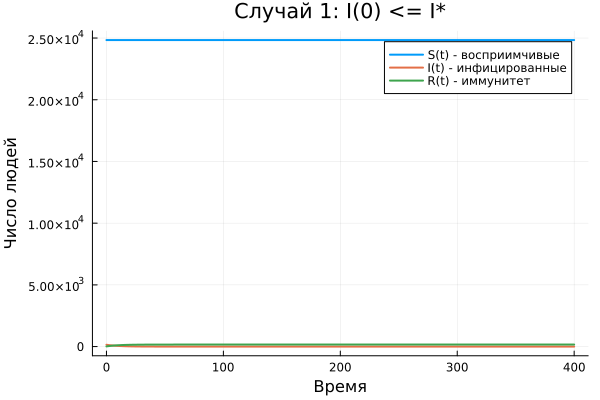
\includegraphics[width=1\linewidth,height=\textheight,keepaspectratio]{image/case1_isolation.png}
\end{column}
\end{columns}
\end{frame}

\begin{frame}{Первый случай: результат}
\protect\phantomsection\label{ux43fux435ux440ux432ux44bux439-ux441ux43bux443ux447ux430ux439-ux440ux435ux437ux443ux43bux44cux442ux430ux442}
При режиме изоляции:

\begin{itemize}
\tightlist
\item
  число восприимчивых практически не меняется;
\item
  инфицированные постепенно выздоравливают;
\item
  количество людей с иммунитетом увеличивается.
\end{itemize}

\[
I(t)\rightarrow0.
\]

\textbf{Эпидемическая вспышка не развивается.}
\end{frame}

\begin{frame}{Второй случай: распространение}
\protect\phantomsection\label{ux432ux442ux43eux440ux43eux439-ux441ux43bux443ux447ux430ux439-ux440ux430ux441ux43fux440ux43eux441ux442ux440ux430ux43dux435ux43dux438ux435}
\begin{columns}[c]
\begin{column}{0.32\linewidth}
\[
I(0)=150
\]

\[
I^*=100
\]

Следовательно,

\[
\boxed{I(0)>I^*}
\]

Инфекция начинает распространяться.
\end{column}

\begin{column}{0.68\linewidth}
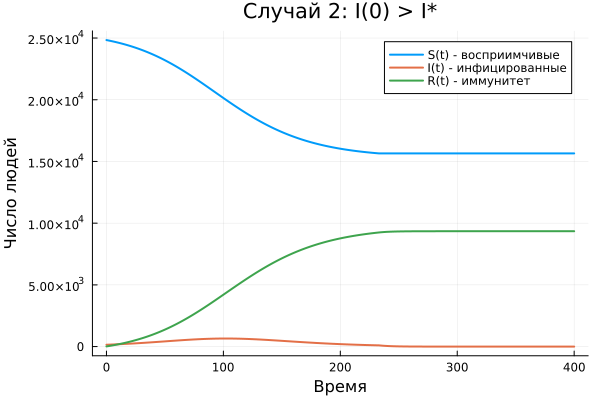
\includegraphics[width=1\linewidth,height=\textheight,keepaspectratio]{image/case2_epidemic.png}
\end{column}
\end{columns}
\end{frame}

\begin{frame}{Второй случай: результат}
\protect\phantomsection\label{ux432ux442ux43eux440ux43eux439-ux441ux43bux443ux447ux430ux439-ux440ux435ux437ux443ux43bux44cux442ux430ux442}
При превышении критического уровня:

\begin{itemize}
\tightlist
\item
  \(S(t)\) уменьшается;
\item
  \(I(t)\) сначала увеличивается;
\item
  после достижения максимума \(I(t)\) уменьшается;
\item
  \(R(t)\) увеличивается.
\end{itemize}

\textbf{Возникает эпидемическая вспышка.}
\end{frame}

\begin{frame}{Сравнение сценариев}
\protect\phantomsection\label{ux441ux440ux430ux432ux43dux435ux43dux438ux435-ux441ux446ux435ux43dux430ux440ux438ux435ux432}
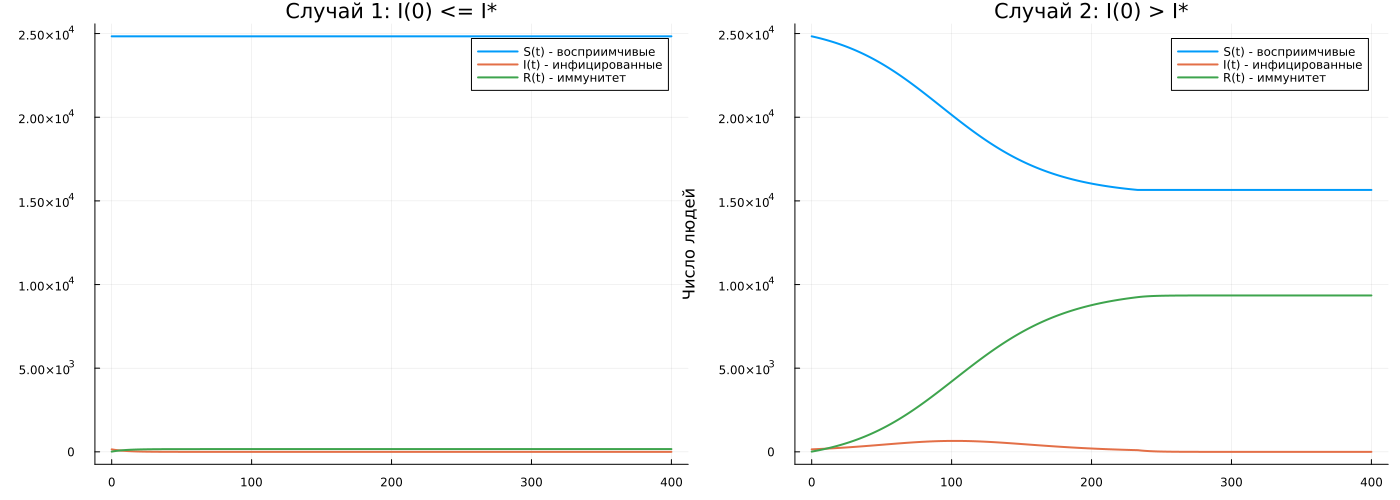
\includegraphics[width=0.78\linewidth,height=\textheight,keepaspectratio]{image/both_cases.png}

Начальные значения населения одинаковы.

\[
I\le I^*
\quad\Rightarrow\quad
\text{режим изоляции},
\]

\[
I>I^*
\quad\Rightarrow\quad
\text{распространение инфекции}.
\]
\end{frame}

\begin{frame}{Итог}
\protect\phantomsection\label{ux438ux442ux43eux433}
Для варианта 2 реализована модель эпидемии с тремя группами населения:

\[
S(t),\qquad I(t),\qquad R(t).
\]

Рассмотрены оба режима:

\begin{itemize}
\tightlist
\item
  \(I(0)\le I^*\) --- новых заражений нет;
\item
  \(I(0)>I^*\) --- инфекция распространяется.
\end{itemize}

Для каждого случая выполнено численное решение и построена динамика всех
трёх групп.

\textbf{Критический уровень \(I^*\) определяет режим развития эпидемии.}
\end{frame}




\end{document}
